\documentclass[a4paper,12pt,twoside]{book}
\usepackage{upca/lesi}
\usepackage{tabularx}
\usepackage{longtable}
\usepackage{caption}
\captionsetup{justification=centering,singlelinecheck=false,position=bottom}
\usepackage{float}
\usepackage[section]{placeins}
\usepackage[figuresright]{rotating}
\usepackage[htt]{hyphenat} % hifenizar texto em \texttt
\setlength{\emergencystretch}{3em}
\usepackage{tikz}
\usetikzlibrary{arrows.meta,calc,positioning,shapes.geometric,fit,backgrounds}
\lstset{literate={á}{{\'a}}1 {à}{{\`a}}1 {ã}{{\~a}}1 {â}{{\^a}}1 {é}{{\'e}}1 {ê}{{\^e}}1 {í}{{\'i}}1 {ó}{{\'o}}1 {õ}{{\~o}}1 {ô}{{\^o}}1 {ú}{{\'u}}1 {ç}{{\c c}}1 {Á}{{\'A}}1 {É}{{\'E}}1}
\usepackage{fancyhdr}
\pagestyle{fancy}
\fancyhf{}
\renewcommand{\headrulewidth}{0pt}
\fancyhead[R]{\slshape\leftmark}
\fancyfoot[C]{\thepage}
\fancypagestyle{plain}{\fancyhf{}\renewcommand{\headrulewidth}{0pt}\fancyfoot[C]{\thepage}}
\newcommand{\porcompletar}[1]{\par\medskip\noindent\textcolor{red}{[A completar: #1]}\par\medskip}

% Paleta da aplicação (wwwroot/css/app.css, tema claro e escuro)
% Paleta cromática da aplicação, copiada de GamP-SCPeriop/wwwroot/css/app.css.
% Tema claro (:root)
\definecolor{gBrand}{HTML}{6A96A6}
\definecolor{gBrandDark}{HTML}{4D7686}
\definecolor{gInk}{HTML}{26343C}
\definecolor{gInkSoft}{HTML}{64767D}
\definecolor{gPaper}{HTML}{E9EAEB}
\definecolor{gCard}{HTML}{F6F6F7}
\definecolor{gLine}{HTML}{DADCDD}
\definecolor{gApproved}{HTML}{3F7D5C}
\definecolor{gApprovedBg}{HTML}{E6EFE9}
\definecolor{gReproved}{HTML}{B24949}
\definecolor{gReprovedBg}{HTML}{F5E7E6}
\definecolor{gPendente}{HTML}{C08A3E}
\definecolor{gPendenteBg}{HTML}{F3EADA}
\definecolor{gPorIniciar}{HTML}{7A8B90}
\definecolor{gPorIniciarBg}{HTML}{EBEEEC}
\definecolor{gStar}{HTML}{D9A441}
% Tema escuro ([data-bs-theme="dark"])
\definecolor{gdBrand}{HTML}{8FB6C4}
\definecolor{gdBrandDark}{HTML}{6A96A6}
\definecolor{gdInk}{HTML}{E7E8E9}
\definecolor{gdInkSoft}{HTML}{9DA0A3}
\definecolor{gdPaper}{HTML}{1B1C1E}
\definecolor{gdCard}{HTML}{28292B}
\definecolor{gdLine}{HTML}{3A3B3D}
\definecolor{gdApproved}{HTML}{6FB98D}
\definecolor{gdReproved}{HTML}{D97A7A}
\definecolor{gdPendente}{HTML}{E0B36E}

% Amostra de cor para as tabelas: \amostra{nome}
\newcommand{\amostra}[1]{\tikz[baseline=-0.6ex]\draw[gLine,fill=#1,rounded corners=1.5pt] (0,-0.2) rectangle (0.8,0.2);}


% Estilos BPMN, site map e task model
% Estilos TikZ partilhados pelos diagramas do relatório.

\tikzset{
  % --- BPMN ---
  bpmn/.style={font=\scriptsize, >={Stealth[length=2mm]}},
  tarefa/.style={draw=gInk, fill=white, rounded corners=4pt, minimum width=2.3cm,
    minimum height=1.15cm, text width=2.1cm, align=center, line width=0.6pt},
  tarefasis/.style={tarefa, fill=gBrand!12},
  inicio/.style={draw=gInk, fill=white, circle, minimum size=6.5mm, inner sep=0pt, line width=0.6pt},
  fim/.style={draw=gInk, fill=white, circle, minimum size=6.5mm, inner sep=0pt, line width=2pt},
  intermedio/.style={draw=gInk, fill=white, circle, minimum size=6.5mm, inner sep=0pt,
    line width=0.6pt, double, double distance=1pt},
  gateway/.style={draw=gInk, fill=white, diamond, minimum size=9mm, inner sep=0pt,
    line width=0.6pt, font=\normalsize},
  fluxo/.style={->, draw=gInk, line width=0.6pt},
  rotulo/.style={font=\tiny\itshape, text=gInkSoft, inner sep=1.5pt},
  evento/.style={font=\tiny, text width=2cm, align=center, text=gInk},
  pista/.style={draw=gInkSoft, line width=0.5pt},
  nomepista/.style={font=\scriptsize\bfseries, rotate=90, text=gInk},
  % --- Site map ---
  ecra/.style={draw=#1, fill=#1!10, rounded corners=3pt, font=\scriptsize, align=center,
    minimum height=0.95cm, text width=2.9cm, inner sep=2pt, line width=0.6pt},
  area/.style={draw=#1, fill=#1!4, rounded corners=6pt, line width=0.6pt, inner sep=8pt},
  nomearea/.style={font=\scriptsize\bfseries, text=#1, anchor=north west},
  ligacao/.style={->, >={Stealth[length=1.6mm]}, draw=gInkSoft, line width=0.5pt},
  atalho/.style={ligacao, dashed},
  % --- Task model (HTA) ---
  tarefahta/.style={draw=gInk, fill=gCard, rounded corners=3pt, font=\scriptsize,
    align=center, text width=2.5cm, minimum height=1cm, inner sep=2pt, line width=0.6pt},
  tarefaraiz/.style={tarefahta, fill=gBrand!15, draw=gBrandDark, line width=1pt, text width=4.2cm},
  plano/.style={font=\tiny\itshape, text=gBrandDark, align=left},
}

% Perfis no site map
\colorlet{cPublico}{gPorIniciar}
\colorlet{cAdmin}{gReproved}
\colorlet{cSupervisor}{gBrandDark}
\colorlet{cAluno}{gApproved}
\colorlet{cComum}{gPendente}

% Marcador de gateway exclusivo (X)
\newcommand{\gwx}{$\times$}

% Diagrama BPMN numa página na horizontal (dentro de sidewaysfigure).
% Usa a exportação do modelador se existir (bpmn/<nome>.pdf, depois .png);
% caso contrário, usa o desenho TikZ em figuras/bpmn-<nome>.tex.
\newcommand{\bpmnfigura}[1]{%
  \IfFileExists{bpmn/#1.pdf}{%
    \includegraphics[width=\textheight,height=0.82\textwidth,keepaspectratio]{bpmn/#1.pdf}}{%
  \IfFileExists{bpmn/#1.png}{%
    \includegraphics[width=\textheight,height=0.82\textwidth,keepaspectratio]{bpmn/#1.png}}{%
    \resizebox{\textheight}{!}{\input{figuras/bpmn-#1}}}}}

% Rota de um ecrã, por baixo do nome, no site map
\newcommand{\rota}[1]{\\[-1pt]{\tiny\ttfamily #1}}


\title{GamP-SCPeriop\\[3mm]\large Plataforma de gestão e gamificação de percursos de formação perioperatória}
\author{Sérgio Oliveira (n.º 15656)}
\MEI
\date{Outubro de 2026}

\makeglossaries
\raggedbottom
\titlespacing*{\chapter}{0pt}{15pt}{20pt}
\makeatletter
\renewcommand*{\glsentryfmt}{%
  \ifglsused{\glslabel}{\glsgenentryfmt}{%
    \edef\gamp@gtype{\glsentrytype{\glslabel}}%
    \ifdefstring{\gamp@gtype}{main}{\emph{\glsgenentryfmt}}{\glsgenentryfmt}}}
\makeatother
\setglossarypreamble[main]{Os termos deste glossário aparecem em itálico na primeira vez que são usados no texto.\par\bigskip}

\begin{document}
\frontmatter
\maketitle

\begin{resumo}
\porcompletar{resumo em português (150 a 300 palavras): problema, solução, método e principais resultados.}

\textbf{Palavras-chave:} gamificação; formação perioperatória; gestão de percursos de aprendizagem; Blazor; ASP.NET Core.
\end{resumo}

\begin{abstract}
\porcompletar{abstract in English, translated from the Portuguese summary.}

\textbf{Keywords:} gamification; perioperative training; learning pathway management; Blazor; ASP.NET Core.
\end{abstract}


\tableofcontents
\listoffigures
\listoftables

\newacronym{api}{API}{Application Programming Interface (Interface de Programação de Aplicações)}

\newacronym{bpmn}{BPMN}{Business Process Model and Notation}

\newacronym{hta}{HTA}{Hierarchical Task Analysis (Análise Hierárquica de Tarefas)}

\newacronym{jwt}{JWT}{JSON Web Token}

\newacronym{pdf}{PDF}{Portable Document Format}

\newacronym{rest}{REST}{Representational State Transfer}

\newacronym{rgpd}{RGPD}{Regulamento Geral sobre a Proteção de Dados}

\newacronym{spa}{SPA}{Single-Page Application (Aplicação de Página Única)}

\newacronym{wcag}{WCAG}{Web Content Accessibility Guidelines}

\printglossary[type=\acronymtype,title={Siglas \& Acrónimos}]

\newglossaryentry{percurso}
{
    name=percurso,
    description={Plano de estudo de um grupo de supervisionados, dividido em módulos e componentes, com datas e critérios de aprovação. Pertence a um supervisor}
}

\newglossaryentry{molde}
{
    name=molde,
    description={Estrutura-base de um percurso (módulos, componentes e badges), a partir da qual se criam percursos por clonagem}
}

\newglossaryentry{componente}
{
    name=componente,
    description={Tarefa teórica ou prática dentro de um módulo, associada a uma fase de aprendizagem e com um peso. Pode ter subcomponentes}
}

\newglossaryentry{inscricao}
{
    name=inscrição,
    description={Ligação entre um supervisionado e um percurso. Ao inscrever, o sistema cria uma cópia própria dos módulos do percurso para esse aluno}
}

\newglossaryentry{badge}
{
    name=badge,
    sort=badge,
    description={Conquista atribuída automaticamente a um supervisionado quando atinge uma meta do percurso, por exemplo concluir um módulo}
}

\newglossaryentry{supervisionado}
{
    name=supervisionado,
    description={Estudante ou profissional em formação acompanhado por um supervisor num percurso}
}

\printglossary

\mainmatter

\chapter{Introdução}

A formação em enfermagem perioperatória combina teoria com observação e prática em bloco operatório, ao longo de semanas e sob a orientação de um supervisor. Este documento apresenta a análise e o desenho do \emph{GamP-SCPeriop}, uma aplicação web que organiza esses planos de formação e acrescenta-lhes um sistema de recompensas para motivar os estudantes.

\section{Problema}

Os planos de formação perioperatória são geridos, hoje, em documentos e folhas de cálculo dispersos. Cada supervisor monta o plano de cada estudante à mão, regista as avaliações em papel e calcula o progresso quando precisa dele. Deste processo resultam problemas recorrentes:

\begin{itemize}
    \item Trabalho repetido: planos semelhantes são reescritos para cada grupo e para cada estudante;
    \item Falta de visibilidade: o supervisor não tem uma visão do progresso de todos os seus estudantes, e o estudante não sabe onde está no seu plano;
    \item Avaliação pouco estruturada: os critérios e as fases de aprendizagem variam de supervisor para supervisor;
    \item Pouca motivação: um plano longo, sem marcos visíveis, torna-se monótono para quem o percorre.
\end{itemize}

\section{Solução proposta}

O GamP-SCPeriop estrutura cada plano como um \gls{percurso}, dividido em módulos e \glspl{componente}, e associa cada componente a uma das cinco fases de aprendizagem, da teoria à prática supervisionada. Os percursos são criados a partir de \glspl{molde}, o que evita reescrever estruturas comuns. Cada \gls{supervisionado} recebe uma cópia própria do percurso, que o supervisor pode ajustar sem alterar o percurso dos restantes.

O supervisor avalia cada componente numa escala qualitativa de seis estados, e o sistema calcula automaticamente o progresso do estudante. Quando o estudante atinge uma meta, recebe uma \gls{badge} e uma notificação.


\section{Objetivos}

Os objetivos deste trabalho são:

\begin{enumerate}
    \item Analisar o processo de formação e avaliação e modelá-lo em \gls{bpmn};
    \item Definir os requisitos funcionais e não funcionais da aplicação;
    \item Caracterizar o utilizador principal e modelar a sua tarefa principal;
    \item Organizar os conteúdos e os ecrãs da aplicação num site map;
    \item Documentar o sistema visual da aplicação;
    \item Descrever a arquitetura, as rotas e os endpoints da \gls{api}.
\end{enumerate}

\section{Âmbito}

O trabalho cobre a aplicação web, nas suas três áreas de acesso: administração, supervisão e área do supervisionado. A aplicação é uma \gls{spa} em Blazor WebAssembly, servida por uma \gls{api} \gls{rest} em ASP.NET Core sobre SQL Server. Ficam fora do âmbito a integração com sistemas académicos e a criação de contas pelos próprios estudantes.

\porcompletar{unidade curricular, docente e restantes elementos do grupo, se aplicável.}

\section{Estrutura do documento}

O Capítulo~\ref{cap:analise} descreve os processos de negócio em \gls{bpmn}, os perfis de acesso e os requisitos. O Capítulo~\ref{cap:utilizador} caracteriza o utilizador principal e modela a sua tarefa. O Capítulo~\ref{cap:sitemap} apresenta o site map, e o Capítulo~\ref{cap:visual} o sistema visual. O Capítulo~\ref{cap:arquitetura} descreve a arquitetura, as rotas e os endpoints. O Capítulo~\ref{cap:conclusao} conclui.

\chapter{Análise do problema}
\label{cap:analise}

Este capítulo descreve o contexto em que a aplicação é usada, os dois processos de negócio que ela suporta, os perfis de acesso e os requisitos.

\section{Contexto e pressupostos}

A aplicação destina-se a uma instituição de ensino que acompanha estudantes em formação perioperatória. Os pressupostos assumidos no desenho estão na Tabela~\ref{tab:pressupostos}.

\begin{table}[H]
    \centering
    \small
    \begin{tabularx}{\linewidth}{lX}
        \toprule
        \textbf{Tema} & \textbf{Pressuposto} \\
        \midrule
        Contas & As contas são criadas pelo administrador; não há registo livre de estudantes. \\
        \midrule
        Instituição & Uma instalação serve uma instituição; por omissão, a Universidade do Minho. \\
        \midrule
        Fases & Cada componente pertence a uma de cinco fases: teórica, observação passiva, observação participada, prática assistida e prática supervisionada. \\
        \midrule
        Avaliação & A avaliação é qualitativa, por componente, e só as fases práticas (assistida e supervisionada) contam para o progresso. \\
        \midrule
        Planos & Cada estudante tem uma cópia própria do percurso, que pode divergir do percurso do grupo. \\
        \bottomrule
    \end{tabularx}
    \caption{Pressupostos assumidos no desenho.}
    \label{tab:pressupostos}
\end{table}

\section{Processos de negócio}

Os processos estão modelados em \gls{bpmn}~\citep{omg-bpmn}. Em cada diagrama, as tarefas a branco são feitas por uma pessoa e as tarefas a azul são feitas automaticamente pelo sistema.

\subsection{Preparar um percurso e inscrever os supervisionados}

Quando um supervisor recebe um novo grupo, cria um percurso a partir de um \gls{molde}. Se não existir um molde adequado, o administrador cria-o primeiro. O sistema copia para o novo percurso os módulos, as componentes e as badges do molde, e o supervisor ajusta o resultado e as datas de cada fase (Figura~\ref{fig:bpmn-percurso}).

\begin{sidewaysfigure}
    \centering
    \bpmnfigura{percurso}
    \caption{Preparar um percurso e inscrever os supervisionados, em BPMN.}
    \label{fig:bpmn-percurso}
\end{sidewaysfigure}

Ao inscrever cada supervisionado, o sistema faz uma segunda cópia, desta vez do percurso para a \gls{inscricao}. É esta cópia que o supervisor ajusta quando um estudante precisa de um plano diferente (modo \emph{Individual} do construtor de percursos), sem alterar o percurso do grupo (modo \emph{Geral}) nem o molde.

\subsection{Avaliar um supervisionado e atribuir badges}

Depois de uma sessão prática, o supervisor abre a ficha de avaliação do estudante e classifica as componentes, módulo a módulo e fase a fase. Ao guardar, o sistema recalcula o progresso e verifica se o estudante ganhou alguma \gls{badge} (Figura~\ref{fig:bpmn-avaliacao}).

\begin{sidewaysfigure}
    \centering
    \bpmnfigura{avaliacao}
    \caption{Avaliar um supervisionado e atribuir badges, em BPMN.}
    \label{fig:bpmn-avaliacao}
\end{sidewaysfigure}

Cada componente recebe um de seis estados (Tabela~\ref{tab:estados}). O progresso do percurso é a percentagem de componentes avaliáveis em \emph{Acima da média} ou \emph{Consistente}. São avaliáveis as componentes das fases práticas, com peso maior que zero, que não tenham subcomponentes. O mesmo cálculo é feito para cada módulo cuja avaliação mudou.

\begin{table}[H]
    \centering
    \small
    \begin{tabularx}{\linewidth}{llX}
        \toprule
        \textbf{Estado} & \textbf{Cor} & \textbf{Conta como concluída} \\
        \midrule
        Pendente & Cinzento & Não \\
        Em progresso & Azul & Não \\
        Inconsistente & Vermelho & Não \\
        Abaixo da média & Laranja & Não \\
        Acima da média & Amarelo & Sim \\
        Consistente & Verde & Sim \\
        \bottomrule
    \end{tabularx}
    \caption{Estados de avaliação de uma componente.}
    \label{tab:estados}
\end{table}

Há duas regras de atribuição de badges em funcionamento: uma badge de módulo quando o módulo atinge 65\%, e uma badge de percurso quando o percurso atinge 100\%. Cada badge é atribuída uma única vez a cada estudante. Em todos os casos, o estudante recebe uma notificação com uma ligação para a página correspondente.

\section{Atores e perfis de acesso}

A aplicação tem três perfis, apresentados na Tabela~\ref{tab:perfis}. Cada utilizador tem um único perfil, e depois de entrar na aplicação é encaminhado para a página inicial desse perfil.

\begin{table}[H]
    \centering
    \small
    \begin{tabularx}{\linewidth}{lX}
        \toprule
        \textbf{Perfil} & \textbf{O que pode fazer} \\
        \midrule
        Administrador & Gere as contas de supervisores e supervisionados, os moldes de percurso e as badges de cada molde. \\
        \midrule
        Supervisor & Cria e ajusta os seus percursos, inscreve supervisionados, ajusta o plano de cada um e avalia as suas componentes. \\
        \midrule
        Supervisionado & Consulta os seus percursos, módulos, componentes e documentos, o seu progresso e as suas badges; descarrega o relatório global de avaliação. \\
        \bottomrule
    \end{tabularx}
    \caption{Perfis de acesso.}
    \label{tab:perfis}
\end{table}

\section{Requisitos}

Os requisitos estão agrupados por área funcional. Os requisitos não funcionais estão agrupados pelas categorias pedidas: usabilidade, acessibilidade, desempenho, segurança, compatibilidade e adaptação a diferentes dispositivos.

\subsection{Requisitos funcionais}

\begingroup\small
\begin{longtable}{lp{0.84\linewidth}}
\toprule
\textbf{Id} & \textbf{Requisito} \\
\midrule
\endfirsthead
\toprule
\textbf{Id} & \textbf{Requisito} \\
\midrule
\endhead
\bottomrule
\endfoot
\bottomrule
\caption{Requisitos funcionais.}\label{tab:rf}\\
\endlastfoot
\multicolumn{2}{l}{\textbf{Autenticação e contas}} \\
RF01 & Autenticar o utilizador com email e palavra-passe e encaminhá-lo para a página inicial do seu perfil. \\
RF02 & Permitir a qualquer utilizador alterar a sua palavra-passe. \\
RF03 & Permitir ao administrador criar contas de supervisores e de supervisionados. \\
RF04 & Permitir ao administrador repor a palavra-passe de um utilizador. \\
\midrule
\multicolumn{2}{l}{\textbf{Moldes}} \\
RF05 & Gerir moldes de percurso: criar, consultar e apagar. \\
RF06 & Gerir os módulos de um molde, com peso e ordem. \\
RF07 & Gerir as componentes de um módulo do molde: título, descrição, fase, peso, ordem, documento \gls{pdf} e subcomponentes. \\
RF08 & Gerir as badges de um molde: nome, descrição, ícone, cor, nível de raridade e regra de atribuição. \\
RF09 & Carregar documentos \gls{pdf} e associá-los a componentes. \\
\midrule
\multicolumn{2}{l}{\textbf{Percursos e inscrições}} \\
RF10 & Criar um percurso vazio ou a partir de um molde, copiando os seus módulos, componentes e badges. \\
RF11 & Editar um percurso: título, datas, módulos, componentes, pesos e ordem. \\
RF12 & Definir as datas de início e fim de cada fase em cada módulo. \\
RF13 & Apagar um percurso. \\
RF14 & Inscrever um supervisionado num percurso, criando uma cópia própria dos módulos; impedir inscrições repetidas. \\
RF15 & Ajustar o plano de um supervisionado sem alterar o percurso do grupo nem o molde. \\
RF16 & Marcar inscrições como favoritas e ocultá-las do painel do supervisor. \\
\midrule
\multicolumn{2}{l}{\textbf{Avaliação}} \\
RF17 & Classificar cada componente de um supervisionado com um dos seis estados da Tabela~\ref{tab:estados}. \\
RF18 & Recalcular o progresso do percurso e de cada módulo afetado sempre que uma avaliação é guardada. \\
RF19 & Gerar o relatório global de avaliação de um supervisionado em \gls{pdf}. \\
\midrule
\multicolumn{2}{l}{\textbf{Gamificação e notificações}} \\
RF20 & Atribuir uma badge de módulo quando o módulo atinge 65\% de progresso. \\
RF21 & Atribuir uma badge de percurso quando o percurso atinge 100\% de progresso. \\
RF22 & Atribuir cada badge uma única vez a cada supervisionado, com a data em que foi obtida. \\
RF23 & Notificar o supervisionado de cada nova avaliação e de cada nova badge, com uma ligação para a página correspondente. \\
RF24 & Mostrar o número de notificações por ler e permitir marcá-las como lidas. \\
\midrule
\multicolumn{2}{l}{\textbf{Consulta}} \\
RF25 & Mostrar ao supervisor os seus percursos, o número de supervisionados de cada um e o progresso de cada supervisionado. \\
RF26 & Mostrar ao supervisionado os seus percursos, módulos, componentes, documentos e progresso. \\
RF27 & Mostrar ao supervisionado as badges obtidas e as que ainda pode obter. \\
\end{longtable}
\endgroup

\subsection{Requisitos não funcionais}

\begingroup\small
\begin{longtable}{lp{0.84\linewidth}}
\toprule
\textbf{Id} & \textbf{Requisito} \\
\midrule
\endfirsthead
\toprule
\textbf{Id} & \textbf{Requisito} \\
\midrule
\endhead
\bottomrule
\endfoot
\bottomrule
\caption{Requisitos não funcionais.}\label{tab:rnf}\\
\endlastfoot
\multicolumn{2}{l}{\textbf{Usabilidade}} \\
RNF01 & \textbf{Avaliação num só ecrã.} O supervisor avalia todas as componentes de um estudante num único ecrã, agrupadas por módulo e por fase. \\
RNF02 & \textbf{Gravação explícita.} As classificações só são gravadas quando o supervisor confirma; o botão de gravar fica inativo enquanto não houver alterações. \\
RNF03 & \textbf{Consistência.} Os estados de avaliação usam as mesmas cores e os mesmos nomes em todos os ecrãs. \\
RNF04 & \textbf{Visibilidade do progresso.} O progresso é mostrado em barra e em percentagem no painel do supervisor e na área do supervisionado. \\
\midrule
\multicolumn{2}{l}{\textbf{Acessibilidade}} \\
RNF05 & \textbf{Contraste.} O texto cumpre o contraste mínimo de 4,5:1 das \gls{wcag} 2.2, nível AA~\citep{w3c-wcag22}, nos temas claro e escuro. \\
RNF06 & \textbf{Cor não é a única pista.} Cada estado de avaliação é identificado por cor e por texto. \\
RNF07 & \textbf{Teclado e leitores de ecrã.} Todas as ações podem ser feitas com o teclado, e os botões só com ícone têm um nome acessível. \\
\midrule
\multicolumn{2}{l}{\textbf{Desempenho}} \\
RNF08 & \textbf{Navegação sem recarregar.} Depois do primeiro carregamento, a navegação entre ecrãs não recarrega a página. \\
RNF09 & \textbf{Um pedido por gravação.} Guardar uma avaliação, recalcular o progresso e atribuir badges é feito num único pedido ao servidor. \\
\midrule
\multicolumn{2}{l}{\textbf{Segurança}} \\
RNF10 & \textbf{Palavras-passe.} As palavras-passe são guardadas apenas como hash BCrypt e nunca são devolvidas pela \gls{api}. \\
RNF11 & \textbf{Autenticação.} Todos os pedidos à \gls{api}, exceto a autenticação, exigem um \gls{jwt} válido, assinado pelo servidor e com validade limitada. \\
RNF12 & \textbf{Autorização no servidor.} O servidor verifica o perfil e a posse dos dados em cada pedido: um supervisionado só acede aos seus dados e um supervisor só aos dos seus percursos. \\
RNF13 & \textbf{Documentos protegidos.} Os documentos carregados só podem ser descarregados por utilizadores autenticados. \\
RNF14 & \textbf{Dados pessoais.} Só são guardados os dados pessoais necessários (nome, email, instituição), em conformidade com o \gls{rgpd}. \\
\midrule
\multicolumn{2}{l}{\textbf{Compatibilidade}} \\
RNF15 & \textbf{Navegadores.} A aplicação funciona nas versões atuais do Chrome, Edge, Firefox e Safari, que suportam WebAssembly. \\
RNF16 & \textbf{Interoperabilidade.} A \gls{api} \gls{rest} está descrita em OpenAPI e pode ser explorada em \texttt{/swagger} em desenvolvimento. \\
\midrule
\multicolumn{2}{l}{\textbf{Adaptação a diferentes dispositivos}} \\
RNF17 & \textbf{Layout adaptável.} Os ecrãs adaptam-se a telemóvel (menos de 576~px), tablet e computador (a partir de 1200~px), sem deslocamento horizontal da página. \\
RNF18 & \textbf{Temas.} A aplicação oferece um tema claro e um tema escuro, escolhidos pelo utilizador. \\
RNF19 & \textbf{Instalação.} A aplicação pode ser instalada como aplicação web progressiva, com ícone e nome próprios. \\
\end{longtable}
\endgroup

\chapter{Utilizador e task model principal}
\label{cap:utilizador}

O utilizador principal é o supervisor, porque é ele quem cria os percursos, acompanha os estudantes e alimenta, com as suas avaliações, o progresso e as badges que os estudantes veem. Sem a sua atividade regular, a área do supervisionado fica vazia.

\section{Utilizador principal}

A Tabela~\ref{tab:utilizador} resume o perfil-tipo do supervisor.

\begin{table}[H]
    \centering
    \small
    \begin{tabularx}{\linewidth}{lX}
        \toprule
        \textbf{Aspeto} & \textbf{Descrição} \\
        \midrule
        Quem é & Enfermeiro ou docente que orienta estudantes em contexto de bloco operatório, normalmente vários em simultâneo e em percursos diferentes. \\
        \midrule
        Características & Domina a matéria clínica e os critérios de avaliação; tem competência digital média; tem pouco tempo entre turnos; usa o computador do serviço e, por vezes, um tablet ou telemóvel. \\
        \midrule
        Necessidades & Montar planos sem os reescrever de raiz; ver de relance em que ponto está cada estudante; registar avaliações logo após a sessão prática, de forma rápida e sem ambiguidade. \\
        \midrule
        Objetivos & Garantir que cada estudante passa por todas as fases de aprendizagem dentro dos prazos; ter um registo das avaliações que possa justificar; manter os estudantes motivados ao longo do percurso. \\
        \midrule
        Frustrações atuais & Folhas de cálculo diferentes para cada grupo; progresso calculado à mão; avaliações em papel que se perdem ou ficam por registar. \\
        \bottomrule
    \end{tabularx}
    \caption{Perfil do utilizador principal: o supervisor.}
    \label{tab:utilizador}
\end{table}

O supervisionado é um utilizador secundário: consulta o seu plano e o seu progresso, mas não altera dados. O administrador usa a aplicação com pouca frequência, sobretudo no início de cada ano letivo.

\section{Tarefa principal}

A tarefa principal é \textbf{avaliar um supervisionado após uma sessão prática}. É a tarefa mais frequente do supervisor e é ela que faz avançar o progresso do estudante e que desencadeia a atribuição de badges (Figura~\ref{fig:bpmn-avaliacao}).

A Figura~\ref{fig:task-model} decompõe a tarefa numa análise hierárquica de tarefas (\gls{hta})~\citep{annett-hta}. Cada nível divide a tarefa de cima em passos mais concretos, e os planos indicam a ordem em que esses passos são feitos.

\begin{figure}[H]
    \centering
    \resizebox{\linewidth}{!}{% Task model (HTA): avaliar um supervisionado após uma sessão prática.
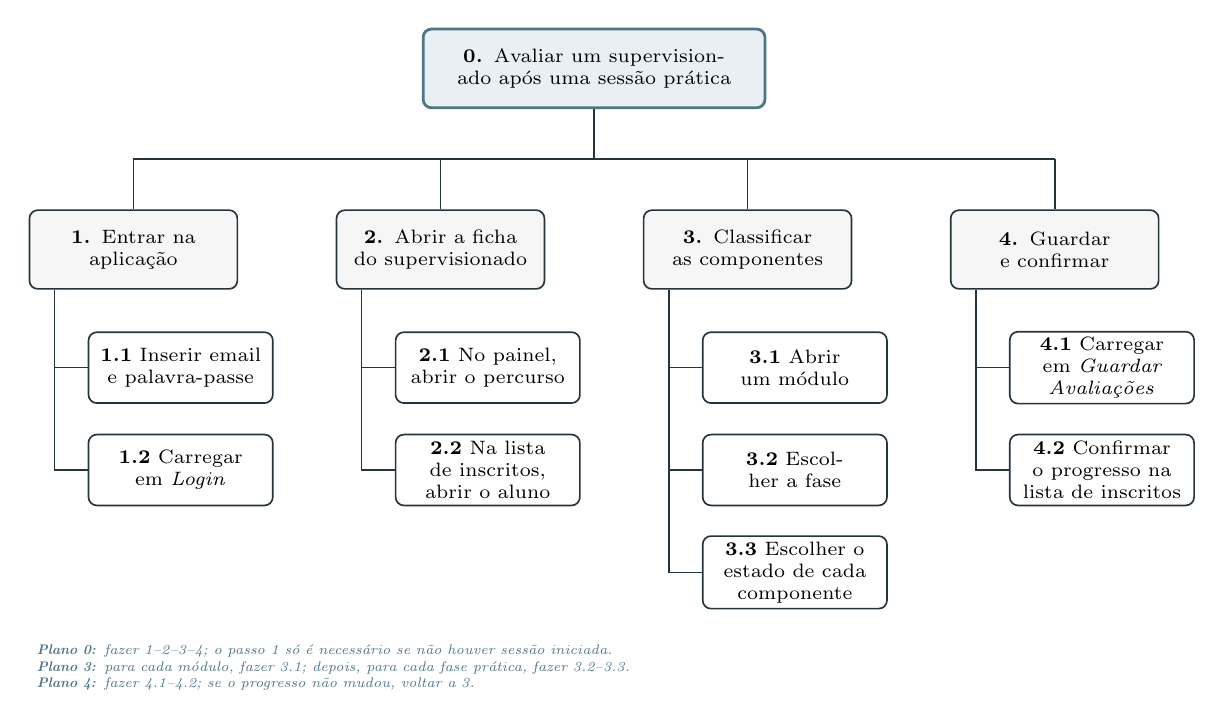
\begin{tikzpicture}[sub/.style={tarefahta, fill=white, text width=2.2cm, minimum height=0.9cm}]
  % Tarefa principal
  \node[tarefaraiz] (r) at (5.85,2.3) {\textbf{0.} Avaliar um supervisionado após uma sessão prática};

  % Subtarefas
  \node[tarefahta] (n1) at (0,0)    {\textbf{1.} Entrar na aplicação};
  \node[tarefahta] (n2) at (3.9,0)  {\textbf{2.} Abrir a ficha do supervisionado};
  \node[tarefahta] (n3) at (7.8,0)  {\textbf{3.} Classificar as componentes};
  \node[tarefahta] (n4) at (11.7,0) {\textbf{4.} Guardar e confirmar};

  \draw[gInk, line width=0.6pt] (r.south) -- (5.85,1.15);
  \draw[gInk, line width=0.6pt] (0,1.15) -- (11.7,1.15);
  \foreach \nd/\x in {n1/0, n2/3.9, n3/7.8, n4/11.7}
    \draw[gInk, line width=0.6pt] (\x,1.15) -- (\nd.north);

  % Ações
  \node[sub] (c11) at (0.6,-1.5)  {\textbf{1.1} Inserir email e palavra-passe};
  \node[sub] (c12) at (0.6,-2.8)  {\textbf{1.2} Carregar em \emph{Login}};

  \node[sub] (c21) at (4.5,-1.5)  {\textbf{2.1} No painel, abrir o percurso};
  \node[sub] (c22) at (4.5,-2.8)  {\textbf{2.2} Na lista de inscritos, abrir o aluno};

  \node[sub] (c31) at (8.4,-1.5)  {\textbf{3.1} Abrir um módulo};
  \node[sub] (c32) at (8.4,-2.8)  {\textbf{3.2} Escolher a fase};
  \node[sub] (c33) at (8.4,-4.1)  {\textbf{3.3} Escolher o estado de cada componente};

  \node[sub] (c41) at (12.3,-1.5) {\textbf{4.1} Carregar em \emph{Guardar Avaliações}};
  \node[sub] (c42) at (12.3,-2.8) {\textbf{4.2} Confirmar o progresso na lista de inscritos};

  \begin{scope}[gInk, line width=0.5pt]
    \draw ($(n1.south)+(-1.0,0)$) |- (c11.west);
    \draw ($(n1.south)+(-1.0,0)$) |- (c12.west);
    \draw ($(n2.south)+(-1.0,0)$) |- (c21.west);
    \draw ($(n2.south)+(-1.0,0)$) |- (c22.west);
    \draw ($(n3.south)+(-1.0,0)$) |- (c31.west);
    \draw ($(n3.south)+(-1.0,0)$) |- (c32.west);
    \draw ($(n3.south)+(-1.0,0)$) |- (c33.west);
    \draw ($(n4.south)+(-1.0,0)$) |- (c41.west);
    \draw ($(n4.south)+(-1.0,0)$) |- (c42.west);
  \end{scope}

  % Planos
  \node[plano, anchor=north west, text width=14.5cm] at (-1.35,-4.9) {%
    \textbf{Plano 0:} fazer 1--2--3--4; o passo 1 só é necessário se não houver sessão iniciada.\\
    \textbf{Plano 3:} para cada módulo, fazer 3.1; depois, para cada fase prática, fazer 3.2--3.3.\\
    \textbf{Plano 4:} fazer 4.1--4.2; se o progresso não mudou, voltar a 3.};
\end{tikzpicture}
}
    \caption{Task model da tarefa principal, em HTA.}
    \label{fig:task-model}
\end{figure}

A sequência de ações, a partir do ecrã de entrada, é a seguinte:

\begin{enumerate}
    \item Na página de entrada, o supervisor insere o email e a palavra-passe e carrega em \emph{Login}; a aplicação abre o painel do supervisor (\texttt{/dashboard}).
    \item No painel, carrega no cartão do percurso; abre-se a gestão do percurso, com a lista de supervisionados inscritos (\texttt{/pathway/\{id\}/students}).
    \item Na lista, carrega no estudante; abre-se a ficha de avaliação (\texttt{/evaluate/\{id\}}).
    \item Na ficha, abre um módulo, escolhe a fase prática e, para cada componente, carrega num dos estados: \emph{Inconsistente}, \emph{Abaixo da média}, \emph{Acima da média} ou \emph{Consistente}.
    \item Repete o passo anterior para cada fase e cada módulo que avaliou na sessão.
    \item Carrega em \emph{Guardar Avaliações}. O sistema grava as classificações, recalcula o progresso, atribui as badges devidas e notifica o estudante.
    \item Volta à lista de inscritos e confirma o novo valor de \emph{Progresso no Percurso}.
\end{enumerate}

Sem contar com a autenticação, a tarefa exige três ecrãs e duas navegações até à ficha de avaliação. O resto do trabalho acontece num único ecrã, como pede o requisito RNF01.

\chapter{Site map}
\label{cap:sitemap}

A aplicação divide-se numa área pública, com a entrada, e numa área autenticada com uma secção por perfil. Depois do login, cada utilizador é levado para a página inicial do seu perfil e só vê os ecrãs dessa secção, mais os que são comuns a todos (Figura~\ref{fig:sitemap}).

\begin{figure}[H]
    \centering
    \resizebox{\linewidth}{!}{% Site map: uma coluna por área de acesso; cada nó é um ecrã, com a rota por baixo.
% Linha cheia = navegação hierárquica; tracejado = atalho entre ecrãs.
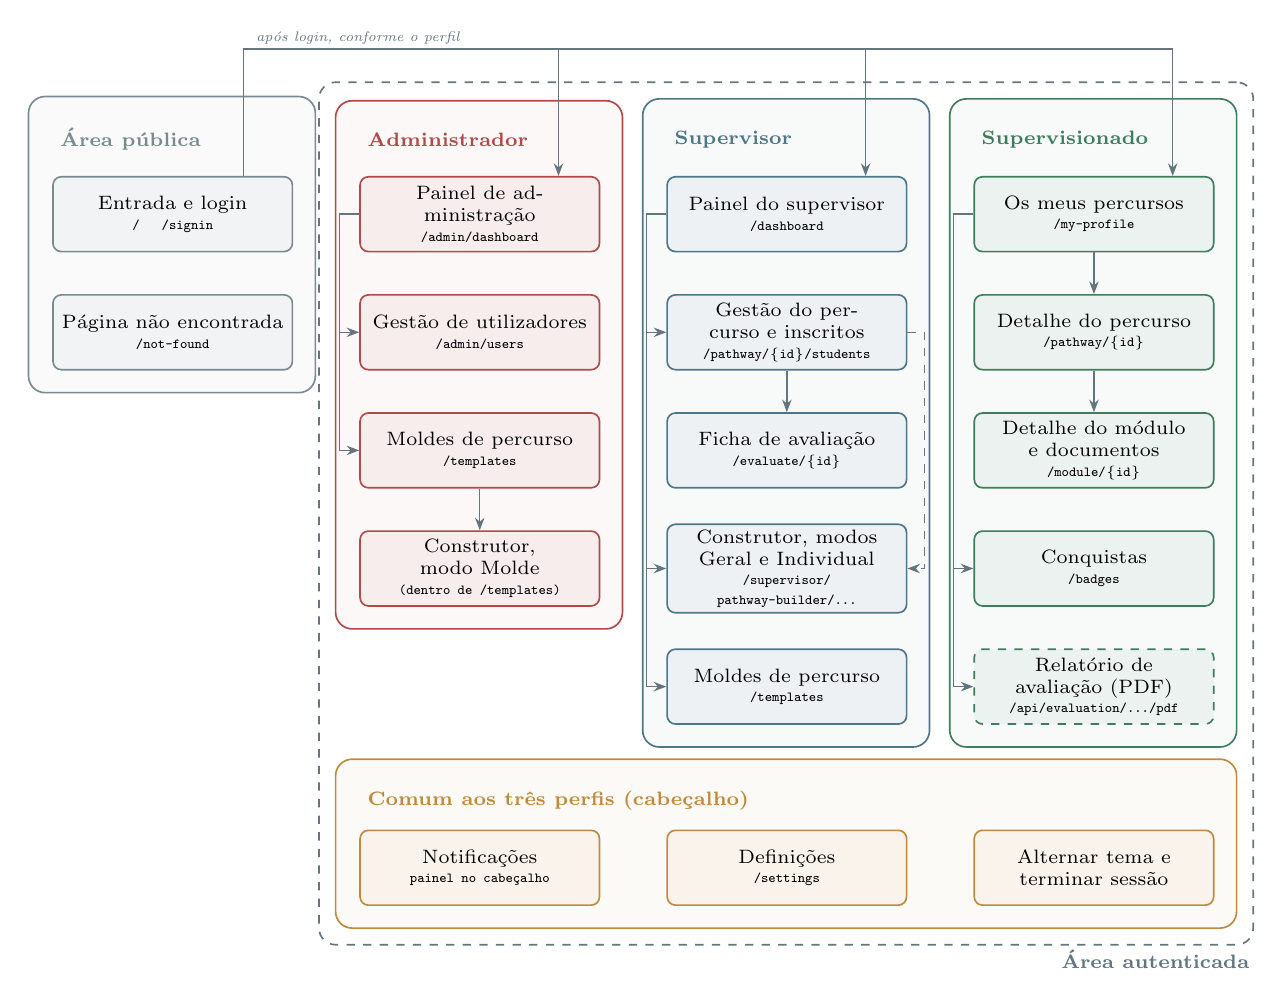
\begin{tikzpicture}[ecra/.append style={text width=2.9cm}]
  % ---------- Área pública ----------
  \node[nomearea=cPublico, anchor=west] (lp) at (-1.55,0.95) {Área pública};
  \node[ecra=cPublico] (p1) at (0,0)    {Entrada e login\rota{/ \ \ /signin}};
  \node[ecra=cPublico] (p2) at (0,-1.5) {Página não encontrada\rota{/not-found}};

  % ---------- Administrador ----------
  \node[nomearea=cAdmin, anchor=west] (la) at (2.35,0.95) {Administrador};
  \node[ecra=cAdmin] (a1) at (3.9,0)    {Painel de administração\rota{/admin/dashboard}};
  \node[ecra=cAdmin] (a2) at (3.9,-1.5) {Gestão de utilizadores\rota{/admin/users}};
  \node[ecra=cAdmin] (a3) at (3.9,-3.0) {Moldes de percurso\rota{/templates}};
  \node[ecra=cAdmin] (a4) at (3.9,-4.5) {Construtor, modo Molde\rota{(dentro de /templates)}};

  % ---------- Supervisor ----------
  \node[nomearea=cSupervisor, anchor=west] (ls) at (6.25,0.95) {Supervisor};
  \node[ecra=cSupervisor] (s1) at (7.8,0)    {Painel do supervisor\rota{/dashboard}};
  \node[ecra=cSupervisor] (s2) at (7.8,-1.5) {Gestão do percurso e inscritos\rota{/pathway/\{id\}/students}};
  \node[ecra=cSupervisor] (s3) at (7.8,-3.0) {Ficha de avaliação\rota{/evaluate/\{id\}}};
  \node[ecra=cSupervisor] (s4) at (7.8,-4.5) {Construtor, modos Geral e Individual\rota{/supervisor/}\rota{pathway-builder/\ldots{}}};
  \node[ecra=cSupervisor] (s5) at (7.8,-6.0) {Moldes de percurso\rota{/templates}};

  % ---------- Supervisionado ----------
  \node[nomearea=cAluno, anchor=west] (lu) at (10.15,0.95) {Supervisionado};
  \node[ecra=cAluno] (u1) at (11.7,0)    {Os meus percursos\rota{/my-profile}};
  \node[ecra=cAluno] (u2) at (11.7,-1.5) {Detalhe do percurso\rota{/pathway/\{id\}}};
  \node[ecra=cAluno] (u3) at (11.7,-3.0) {Detalhe do módulo e documentos\rota{/module/\{id\}}};
  \node[ecra=cAluno] (u4) at (11.7,-4.5) {Conquistas\rota{/badges}};
  \node[ecra=cAluno, dashed] (u5) at (11.7,-6.0) {Relatório de avaliação (PDF)\rota{/api/evaluation/\ldots{}/pdf}};

  % ---------- Comum aos perfis autenticados ----------
  \node[nomearea=cComum, anchor=west] (lc) at (2.35,-7.45) {Comum aos três perfis (cabeçalho)};
  \node[ecra=cComum] (c1) at (3.9,-8.3)  {Notificações\rota{painel no cabeçalho}};
  \node[ecra=cComum] (c2) at (7.8,-8.3)  {Definições\rota{/settings}};
  \node[ecra=cComum] (c3) at (11.7,-8.3) {Alternar tema e terminar sessão};

  % ---------- Ligações ----------
  % Login: encaminha para a página inicial de cada perfil
  \draw[ligacao] ($(p1.north)+(0.9,0)$) -- (0.9,2.1) -| ($(a1.north)+(1.0,0)$);
  \draw[ligacao] (0.9,2.1) -| ($(s1.north)+(1.0,0)$);
  \draw[ligacao] (0.9,2.1) -| ($(u1.north)+(1.0,0)$);
  \node[rotulo, anchor=south west] at (1.0,2.1) {após login, conforme o perfil};

  % Administrador
  \draw[ligacao] (a1.west) -- ++(-0.25,0) |- (a2.west);
  \draw[ligacao] (a1.west) -- ++(-0.25,0) |- (a3.west);
  \draw[ligacao] (a3) -- (a4);

  % Supervisor
  \draw[ligacao] (s1.west) -- ++(-0.25,0) |- (s2.west);
  \draw[ligacao] (s1.west) -- ++(-0.25,0) |- (s4.west);
  \draw[ligacao] (s1.west) -- ++(-0.25,0) |- (s5.west);
  \draw[ligacao] (s2) -- (s3);
  \draw[atalho] (s2.east) -- ++(0.22,0) |- (s4.east);

  % Supervisionado
  \draw[ligacao] (u1) -- (u2);
  \draw[ligacao] (u2) -- (u3);
  \draw[ligacao] (u1.west) -- ++(-0.25,0) |- (u4.west);
  \draw[ligacao] (u1.west) -- ++(-0.25,0) |- (u5.west);

  % ---------- Áreas (fundo) ----------
  \begin{scope}[on background layer]
    \node[area=gInkSoft, dashed, fill=none, fit=(la)(lu)(a1)(u5)(c1)(c3), inner sep=14pt] (aut) {};
    \node[rotulo, font=\scriptsize\bfseries, anchor=north east] at (aut.south east) {Área autenticada};
    \node[area=cPublico, fit=(lp)(p1)(p2)] {};
    \node[area=cAdmin, fit=(la)(a1)(a4)] {};
    \node[area=cSupervisor, fit=(ls)(s1)(s5)] {};
    \node[area=cAluno, fit=(lu)(u1)(u5)] {};
    \node[area=cComum, fit=(lc)(c1)(c3)] {};
  \end{scope}
\end{tikzpicture}
}
    \caption{Site map do GamP-SCPeriop. Cada caixa é um ecrã, com a rota por baixo; as setas cheias são a navegação principal e a tracejada um atalho.}
    \label{fig:sitemap}
\end{figure}

\section{Organização dos conteúdos}

Os conteúdos seguem a hierarquia do domínio: um percurso tem módulos, e um módulo tem componentes. O site map reproduz essa hierarquia nas duas áreas que a mostram:

\begin{itemize}
    \item Na área do supervisor, o painel lista os percursos; cada percurso abre a lista de inscritos, e cada inscrito abre a sua ficha de avaliação.
    \item Na área do supervisionado, \emph{Os meus percursos} lista os percursos; cada percurso abre os seus módulos, e cada módulo as suas componentes e documentos.
\end{itemize}

\section{Áreas e diferenças de acesso}

A Tabela~\ref{tab:acessos} indica, para cada área, quem lhe pode aceder e por onde se entra.

\begin{table}[H]
    \centering
    \small
    \begin{tabularx}{\linewidth}{llX}
        \toprule
        \textbf{Área} & \textbf{Acesso} & \textbf{Entrada e ecrãs principais} \\
        \midrule
        Pública & Qualquer visitante & Entrada e login (\texttt{/}); página não encontrada. \\
        \midrule
        Administrador & Perfil Administrador & Painel de administração; gestão de utilizadores; moldes de percurso e respetivo construtor. \\
        \midrule
        Supervisor & Perfil Supervisor & Painel com os percursos; gestão de cada percurso e dos inscritos; ficha de avaliação; construtor de percursos; moldes. \\
        \midrule
        Supervisionado & Perfil Supervisionado & Os meus percursos; detalhe do percurso e do módulo; conquistas; relatório de avaliação em PDF. \\
        \midrule
        Comum & Os três perfis & Notificações e alternância de tema no cabeçalho; definições (alterar a palavra-passe); terminar sessão. \\
        \bottomrule
    \end{tabularx}
    \caption{Áreas da aplicação e respetivo acesso.}
    \label{tab:acessos}
\end{table}

\section{Ligações entre ecrãs}

Além da navegação hierárquica, há três tipos de ligação que atravessam o site map:

\begin{itemize}
    \item \textbf{Construtor de percursos.} É o mesmo ecrã em três modos. O administrador usa-o em modo \emph{Molde}; o supervisor usa-o em modo \emph{Geral}, a partir do painel ou da gestão do percurso, e em modo \emph{Individual}, a partir de um inscrito.
    \item \textbf{Notificações.} Cada notificação leva diretamente ao ecrã a que diz respeito: uma nova avaliação abre o detalhe do percurso, e uma nova badge abre as conquistas.
    \item \textbf{Moldes.} O ecrã de moldes é partilhado pelo administrador, que gere os moldes-base, e pelo supervisor, que os consulta para criar percursos.
\end{itemize}

Os ecrãs abaixo da página inicial de cada perfil têm um botão para voltar ao ecrã de cima, e o cabeçalho é igual em todos os ecrãs autenticados.

\chapter{Sistema visual}
\label{cap:visual}

O sistema visual parte de um azul-acinzentado calmo, adequado a um contexto clínico, e reserva as cores fortes para comunicar o estado da avaliação. Todos os valores deste capítulo foram retirados da folha de estilos da aplicação (\texttt{wwwroot/css/app.css}).

\section{Logótipo e identidade visual}

A aplicação ainda não tem logótipo. O cabeçalho mostra o nome da instituição (\emph{Universidade do Minho}) em texto, e os ícones da aplicação instalável são os ícones por omissão do Blazor.

\porcompletar{logótipo ou símbolo do GamP-SCPeriop, versões para fundo claro e escuro, área de proteção e tamanho mínimo.}

\section{Paleta cromática}

A paleta está definida como variáveis CSS, com um valor para o tema claro e outro para o tema escuro (Tabela~\ref{tab:paleta}). A mudança de tema troca os valores das variáveis, sem alterar os ecrãs.

\begin{table}[H]
    \centering
    \small
    \begin{tabularx}{\linewidth}{lcllX}
        \toprule
        \textbf{Variável} & \textbf{Claro} & \textbf{Hex claro} & \textbf{Hex escuro} & \textbf{Função} \\
        \midrule
        \texttt{-{}-brand} & \amostra{gBrand} & \#6A96A6 & \#8FB6C4 & Cor da marca: ícones do cabeçalho, barras de progresso \emph{em curso}, ligações no tema escuro. \\
        \texttt{-{}-brand-dark} & \amostra{gBrandDark} & \#4D7686 & \#6A96A6 & Texto do estado \emph{em curso} e percentagens de progresso. \\
        \texttt{-{}-ink} & \amostra{gInk} & \#26343C & \#E7E8E9 & Texto principal e títulos. \\
        \texttt{-{}-ink-soft} & \amostra{gInkSoft} & \#64767D & \#9DA0A3 & Texto secundário, legendas e metadados. \\
        \texttt{-{}-paper} & \amostra{gPaper} & \#E9EAEB & \#1B1C1E & Fundo da página. \\
        \texttt{-{}-card-bg} & \amostra{gCard} & \#F6F6F7 & \#28292B & Fundo dos cartões. \\
        \texttt{-{}-line} & \amostra{gLine} & \#DADCDD & \#3A3B3D & Contornos, divisórias e trilho das barras de progresso. \\
        \midrule
        \texttt{-{}-approved} & \amostra{gApproved} & \#3F7D5C & \#6FB98D & Estado positivo: concluído, aprovado, consistente. \\
        \texttt{-{}-reproved} & \amostra{gReproved} & \#B24949 & \#D97A7A & Estado negativo: reprovado, inconsistente. \\
        \texttt{-{}-pendente} & \amostra{gPendente} & \#C08A3E & \#E0B36E & Estado intermédio: em curso, a aguardar. \\
        \texttt{-{}-por-iniciar} & \amostra{gPorIniciar} & \#7A8B90 & \#7A8B90 & Estado neutro: ainda não iniciado. \\
        \texttt{-{}-star} & \amostra{gStar} & \#D9A441 & \#D9A441 & Inscrições favoritas (estrela). \\
        \bottomrule
    \end{tabularx}
    \caption{Paleta cromática da aplicação, com a função de cada cor.}
    \label{tab:paleta}
\end{table}

Cada cor de estado tem uma variante de fundo (\texttt{-{}-approved-bg}, \texttt{-{}-reproved-bg}, \texttt{-{}-pendente-bg} e \texttt{-{}-por-iniciar-bg}), usada nas etiquetas de estado: o texto leva a cor do estado e o fundo a sua variante clara.

Há três desvios à paleta na implementação atual: os botões principais usam o azul \#1B6EC2 do modelo-base do Blazor, que não pertence à paleta; os ecrãs ainda têm 74 códigos de cor escritos diretamente, que não mudam com o tema; e \texttt{-{}-em-curso-bg} só está definida no tema escuro. Propõe-se usar \texttt{-{}-brand-dark} nos botões principais e substituir os códigos diretos pelas variáveis.

\subsection{Função das cores principais}

\begin{itemize}
    \item \textbf{Marca} (\texttt{-{}-brand}, \texttt{-{}-brand-dark}): identifica o que pertence à aplicação ou está em curso, como os ícones do cabeçalho, as ligações e as barras de progresso.
    \item \textbf{Neutros} (\texttt{-{}-ink}, \texttt{-{}-paper}, \texttt{-{}-card-bg}, \texttt{-{}-line}): estruturam a página. O fundo é ligeiramente mais escuro que os cartões, para que estes se destaquem sem precisarem de contornos fortes.
    \item \textbf{Estados} (verde, vermelho, âmbar, cinzento): comunicam o resultado de uma avaliação ou o estado de um percurso. São as únicas cores saturadas da interface, para que um problema se veja de relance.
\end{itemize}

\subsection{Contraste}

A Tabela~\ref{tab:contraste} mostra o contraste das combinações mais usadas, calculado segundo as \gls{wcag} 2.2~\citep{w3c-wcag22}. O requisito RNF05 exige pelo menos 4,5:1 para texto.

\begin{table}[H]
    \centering
    \small
    \begin{tabularx}{\linewidth}{Xrrl}
        \toprule
        \textbf{Texto sobre fundo} & \textbf{Claro} & \textbf{Escuro} & \textbf{Cumpre 4,5:1} \\
        \midrule
        \texttt{-{}-ink} sobre \texttt{-{}-card-bg} & 11,86 & 11,87 & Sim \\
        \texttt{-{}-ink-soft} sobre \texttt{-{}-card-bg} & 4,39 & 5,54 & Só no escuro \\
        \texttt{-{}-brand-dark} sobre \texttt{-{}-card-bg} & 4,57 & 4,52 & Sim \\
        Branco sobre o botão principal (\#1B6EC2) & 5,18 & 5,18 & Sim \\
        \texttt{-{}-approved} sobre \texttt{-{}-approved-bg} & 4,16 & 5,23 & Só no escuro \\
        \texttt{-{}-reproved} sobre \texttt{-{}-reproved-bg} & 4,43 & 4,86 & Só no escuro \\
        \texttt{-{}-pendente} sobre \texttt{-{}-pendente-bg} & 2,53 & 6,83 & Só no escuro \\
        \texttt{-{}-por-iniciar} sobre \texttt{-{}-por-iniciar-bg} & 3,03 & 3,03 & Não \\
        \bottomrule
    \end{tabularx}
    \caption{Contraste das principais combinações de cor.}
    \label{tab:contraste}
\end{table}

No tema claro, as etiquetas de estado e o texto secundário ficam abaixo de 4,5:1. A correção mais simples é escurecer a cor do texto de cada estado (por exemplo, \texttt{-{}-pendente} para um âmbar mais escuro) mantendo os fundos. No tema escuro, \texttt{-{}-por-iniciar-bg} mantém o valor claro, que deve ser substituído por um cinzento escuro.

\section{Tipografia}

A aplicação usa uma única família, a \emph{Plus Jakarta Sans}~\citep{plus-jakarta-sans}, carregada do Google Fonts nos pesos 400, 500, 600 e 700. É uma letra sem serifa, geométrica e muito legível em tamanhos pequenos, o que importa em ecrãs densos como a ficha de avaliação.

\begin{table}[H]
    \centering
    \small
    \begin{tabularx}{\linewidth}{llX}
        \toprule
        \textbf{Uso} & \textbf{Peso} & \textbf{Onde} \\
        \midrule
        Títulos de página e de secção & 700 (bold) & Nome do percurso, títulos dos ecrãs. \\
        Nomes e rótulos & 600 (semibold) & Nomes de módulos e componentes, botões, etiquetas de estado (0,72~rem). \\
        Texto corrente & 400 (regular) & Descrições, listas e formulários. \\
        Texto secundário & 400, cor \texttt{-{}-ink-soft} & Datas, legendas e metadados. \\
        \bottomrule
    \end{tabularx}
    \caption{Utilização da tipografia.}
    \label{tab:tipografia}
\end{table}

Os ícones são da biblioteca \emph{Bootstrap Icons} 1.11.3, em traço simples, coerentes com o peso da letra. As badges usam o mesmo conjunto de ícones (por omissão, \texttt{bi-trophy}).

\section{Grelha, margens e espaçamento}

A disposição assenta na grelha de 12 colunas do Bootstrap 5.3~\citep{bootstrap-grid}, dentro de um contentor centrado cuja largura e margens variam com o ecrã (Tabela~\ref{tab:grelha}).

\begin{table}[H]
    \centering
    \small
    \begin{tabularx}{\linewidth}{lllX}
        \toprule
        \textbf{Ecrã} & \textbf{Largura máxima} & \textbf{Margem interior} & \textbf{Notas} \\
        \midrule
        Telemóvel (< 576 px) & 100\% & 16 px (1 rem) & Letra base reduzida para 14 px (0,875 rem). \\
        Tablet e portátil (576--1199 px) & 960 px & 24 px (1,5 rem) & \\
        Computador ($\geq$ 1200 px) & 1400 px & 32 px (2 rem) & \\
        \bottomrule
    \end{tabularx}
    \caption{Contentor principal por tamanho de ecrã.}
    \label{tab:grelha}
\end{table}

Os princípios de espaçamento são:

\begin{itemize}
    \item \textbf{Escala de 4 px.} Os espaçamentos usam a escala do Bootstrap: 4, 8, 16, 24 e 48~px.
    \item \textbf{Cartões como unidade.} Cada percurso, aluno ou módulo é um cartão com cantos de 16~px, sombra leve e sem contorno. Ao passar o rato, o cartão sobe 5~px para indicar que é clicável.
    \item \textbf{Formas arredondadas.} Etiquetas de estado em forma de pílula (raio 20~px) e barras de progresso com 8~px de altura e cantos arredondados.
\end{itemize}

Os raios dos cantos variam hoje entre 8, 10, 12, 15, 16 e 20~px de ecrã para ecrã. Propõe-se reduzi-los a três valores: 8~px para botões e campos, 16~px para cartões, e forma de pílula para etiquetas.

\chapter{Arquitetura}
\label{cap:arquitetura}

O GamP-SCPeriop é um monólito: um único programa ASP.NET Core serve a aplicação cliente e a \gls{api}, e guarda tudo numa única base de dados. Este capítulo justifica essa escolha, descreve os componentes, explica como são resolvidas as rotas do cliente e da \gls{api}, e apresenta o catálogo completo de endpoints.

\section{Estilo arquitetural}
\label{sec:estilo}

Escolheu-se um monólito com três projetos, em vez de serviços independentes, pelas seguintes razões:

\begin{itemize}
    \item \textbf{Escala.} A aplicação serve uma instituição, com dezenas de supervisores e algumas centenas de estudantes. Não há partes do sistema com cargas tão diferentes que justifiquem escalá-las em separado.
    \item \textbf{Consistência.} As operações principais tocam muitas tabelas de uma só vez: criar um percurso a partir de um molde copia módulos, componentes e badges, e guardar uma avaliação atualiza o progresso e atribui badges. Numa única base de dados, estas operações são transações simples.
    \item \textbf{Equipa e operação.} Um único programa, desenvolvido por uma equipa pequena, é mais simples de testar, de pôr em produção e de manter.
    \item \textbf{Código partilhado.} Cliente e servidor usam as mesmas classes de entidades e de DTOs, definidas uma única vez na biblioteca partilhada.
\end{itemize}

O custo desta escolha é que todas as partes são publicadas em conjunto e que uma falha no servidor afeta toda a aplicação. Para o contexto em causa, esse custo é aceitável.

\section{Componentes}

A solução tem três projetos (Tabela~\ref{tab:projetos}). O servidor aloja o cliente: no primeiro acesso, o navegador descarrega a aplicação Blazor WebAssembly como ficheiros estáticos; a partir daí, a aplicação corre no navegador e só comunica com o servidor através da \gls{api} \gls{rest} (Figura~\ref{fig:arquitetura}).

\begin{table}[H]
    \centering
    \small
    \begin{tabularx}{\linewidth}{lX}
        \toprule
        \textbf{Projeto} & \textbf{Responsabilidade} \\
        \midrule
        \texttt{GamP-SCPeriop} & Cliente Blazor WebAssembly: páginas, layouts, componentes reutilizáveis, estado de autenticação e chamadas à \gls{api}. \\
        \midrule
        \texttt{GamP-SCPeriop.Server} & Servidor ASP.NET Core: aloja o cliente, expõe a \gls{api} \gls{rest}, valida os \gls{jwt}, acede à base de dados com Entity Framework Core e gera os relatórios \gls{pdf} com QuestPDF. \\
        \midrule
        \texttt{GamP-SCPeriop.Shared} & Biblioteca partilhada: entidades, DTOs e enumerações usados pelos dois lados. \\
        \bottomrule
    \end{tabularx}
    \caption{Projetos da solução.}
    \label{tab:projetos}
\end{table}

\begin{figure}[H]
    \centering
    \resizebox{\linewidth}{!}{% Arquitetura do monólito: cliente Blazor WebAssembly, servidor ASP.NET Core e dados.
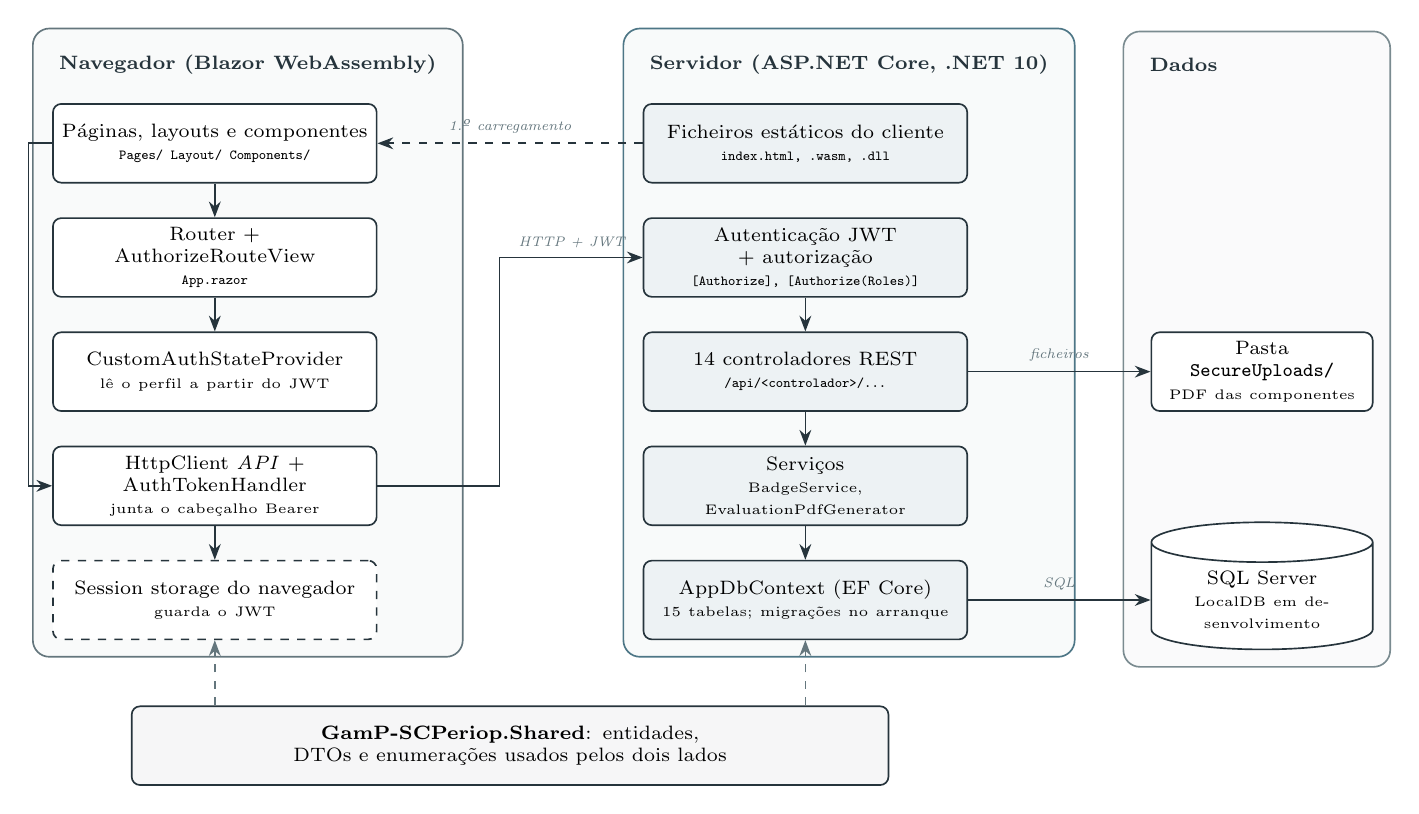
\begin{tikzpicture}[
    comp/.style={draw=gInk, fill=white, rounded corners=3pt, font=\scriptsize, align=center,
      text width=3.9cm, minimum height=1.0cm, inner sep=3pt, line width=0.6pt},
    compsis/.style={comp, fill=gBrand!12},
    titulo/.style={font=\scriptsize\bfseries, text=gInk, anchor=west},
    seta/.style={->, >={Stealth[length=2mm]}, draw=gInk, line width=0.6pt},
    nota/.style={font=\tiny\itshape, text=gInkSoft, align=center},
  ]
  % ---------- Navegador ----------
  \node[titulo] (tc) at (-2.1,4.9) {Navegador (Blazor WebAssembly)};
  \node[comp] (c1) at (0,3.9)   {Páginas, layouts e componentes\\{\tiny\ttfamily Pages/ Layout/ Components/}};
  \node[comp] (c2) at (0,2.45)  {Router +\\AuthorizeRouteView\\{\tiny\ttfamily App.razor}};
  \node[comp] (c3) at (0,1.0)   {CustomAuthStateProvider\\{\tiny lê o perfil a partir do JWT}};
  \node[comp] (c4) at (0,-0.45) {HttpClient \emph{API} +\\AuthTokenHandler\\{\tiny junta o cabeçalho Bearer}};
  \node[comp, dashed] (c5) at (0,-1.9) {Session storage do navegador\\{\tiny guarda o JWT}};

  % ---------- Servidor ----------
  \node[titulo] (ts) at (5.4,4.9) {Servidor (ASP.NET Core, .NET 10)};
  \node[compsis] (s1) at (7.5,3.9)   {Ficheiros estáticos do cliente\\{\tiny\ttfamily index.html, .wasm, .dll}};
  \node[compsis] (s2) at (7.5,2.45)  {Autenticação JWT + autorização\\{\tiny\ttfamily [Authorize], [Authorize(Roles)]}};
  \node[compsis] (s3) at (7.5,1.0)   {14 controladores REST\\{\tiny\ttfamily /api/<controlador>/\ldots}};
  \node[compsis] (s4) at (7.5,-0.45) {Serviços\\{\tiny BadgeService,}\\{\tiny EvaluationPdfGenerator}};
  \node[compsis] (s5) at (7.5,-1.9)  {AppDbContext (EF Core)\\{\tiny 15 tabelas; migrações no arranque}};

  % ---------- Dados ----------
  \node[titulo] (td) at (11.75,4.9) {Dados};
  \node[comp, text width=2.6cm] (d2) at (13.3,1.0) {Pasta \texttt{SecureUploads/}\\{\tiny PDF das componentes}};
  \node[comp, text width=2.6cm, minimum height=1.3cm, cylinder, shape border rotate=90,
        aspect=0.18, rounded corners=0pt] (d1) at (13.3,-1.9) {SQL Server\\{\tiny LocalDB em desenvolvimento}};

  % ---------- Biblioteca partilhada ----------
  \node[comp, text width=9.4cm, fill=gCard] (sh) at (3.75,-3.75)
      {\textbf{GamP-SCPeriop.Shared}: entidades, DTOs e enumerações usados pelos dois lados};

  % ---------- Ligações ----------
  \draw[seta, dashed] (s1.west) -- node[nota, above] {1.º carregamento} (c1.east);
  \draw[seta] (c4.east) -- ++(1.55,0) |- (s2.west);
  \node[nota, anchor=south] at ($(s2.west)+(-0.9,0)$) {HTTP + JWT};
  \draw[seta] (s5.east) -- node[nota, above] {SQL} (d1.west);
  \draw[seta] (s3.east) -- node[nota, above] {ficheiros} (d2.west);
  \draw[seta] (c1) -- (c2);
  \draw[seta] (c2) -- (c3);
  \draw[seta] (c1.west) -- ++(-0.3,0) |- (c4.west);
  \draw[seta] (c4) -- (c5);
  \draw[seta] (s2) -- (s3);
  \draw[seta] (s3) -- (s4);
  \draw[seta] (s4) -- (s5);
  \draw[seta, dashed, gInkSoft] (sh.north -| c5.south) -- (c5.south);
  \draw[seta, dashed, gInkSoft] (sh.north -| s5.south) -- (s5.south);

  % ---------- Fundos ----------
  \begin{scope}[on background layer]
    \node[area=gInkSoft, fit=(tc)(c1)(c5), inner sep=6pt] {};
    \node[area=gBrandDark, fit=(ts)(s1)(s5), inner sep=6pt] {};
    \node[area=gPorIniciar, fit=(td)(d1)(d2), inner sep=6pt] {};
  \end{scope}
\end{tikzpicture}
}
    \caption{Arquitetura do GamP-SCPeriop. A azul, os componentes do servidor; a seta tracejada é o descarregamento inicial da aplicação.}
    \label{fig:arquitetura}
\end{figure}

\subsection{Pipeline do servidor}

Cada pedido atravessa, por esta ordem, os componentes configurados em \texttt{Program.cs}:

\begin{enumerate}
    \item \textbf{CORS}, que aceita pedidos de qualquer origem;
    \item \textbf{Redireção para HTTPS};
    \item \textbf{Ficheiros estáticos}, incluindo os ficheiros da aplicação Blazor (\texttt{UseBlazor\-Framework\-Files} e \texttt{Use\-Static\-Files});
    \item \textbf{Encaminhamento}, que escolhe o controlador e a ação;
    \item \textbf{Autenticação e autorização}, que validam o \gls{jwt} e os atributos \texttt{[Authorize]};
    \item \textbf{Controladores}, e por fim o \textbf{fallback}, que devolve \texttt{index.html} a qualquer pedido que não corresponda a um ficheiro nem a um controlador.
\end{enumerate}

No arranque, o servidor aplica as migrações pendentes à base de dados (32 até à data) e, se não existir nenhum utilizador, cria a conta de administrador inicial. Em desenvolvimento, publica também a documentação OpenAPI em \texttt{/swagger}.

\subsection{Serviços e lógica de negócio}

A lógica de negócio está repartida entre os controladores e dois serviços:

\begin{itemize}
    \item \texttt{BadgeService}: verifica e atribui as badges de módulo e de percurso, e cria as notificações correspondentes;
    \item \texttt{EvaluationPdfGenerator}: gera o relatório global de avaliação de um estudante.
\end{itemize}

As cópias de moldes e de percursos e o cálculo do progresso estão escritos diretamente nos controladores (\texttt{PathwayController}, \texttt{EnrollmentController} e \texttt{EvaluationController}). Mover esta lógica para serviços próprios tornaria o código mais fácil de testar, e é a primeira melhoria proposta para a arquitetura.

\section{Rotas}
\label{sec:rotas}

A aplicação tem dois conjuntos de rotas, resolvidos em lugares diferentes:

\begin{itemize}
    \item \textbf{Rotas do cliente}, como \texttt{/dashboard} ou \texttt{/pathway/7}. São declaradas em cada página com a diretiva \texttt{@page} e resolvidas no navegador pelo \emph{Router} do Blazor. O Capítulo~\ref{cap:sitemap} lista-as todas.
    \item \textbf{Rotas da \gls{api}}, todas começadas por \texttt{/api/}. São declaradas com atributos nos controladores e resolvidas no servidor.
\end{itemize}

A Figura~\ref{fig:rotas} mostra o percurso de um pedido. O servidor tenta, por ordem, servir um ficheiro estático e encontrar um controlador; se nenhum corresponder, devolve \texttt{index.html}, e a aplicação Blazor, já no navegador, escolhe a página.

\begin{figure}[H]
    \centering
    \resizebox{0.82\linewidth}{!}{% Como um URL é resolvido: primeiro pelo servidor, depois (se for o caso) pelo Router do Blazor.
\begin{tikzpicture}[
    passo/.style={draw=gInk, fill=white, rounded corners=3pt, font=\scriptsize, align=center,
      text width=3.0cm, minimum height=0.9cm, inner sep=2pt, line width=0.6pt},
    passosis/.style={passo, fill=gBrand!12},
    decisao/.style={draw=gInk, fill=white, diamond, aspect=2.2, font=\scriptsize, align=center,
      inner sep=1pt, text width=2.0cm, line width=0.6pt},
    fim/.style={passo, fill=gApprovedBg, draw=gApproved},
    erro/.style={passo, fill=gReprovedBg, draw=gReproved},
    seta/.style={->, >={Stealth[length=2mm]}, draw=gInk, line width=0.6pt},
    rot/.style={font=\tiny\itshape, text=gInkSoft, inner sep=1.5pt},
    zona/.style={font=\scriptsize\bfseries, text=gInk, anchor=west},
  ]
  \node[passo] (p0) at (0,0) {Pedido do navegador\\{\tiny\ttfamily GET /pathway/7}};

  % ---- Servidor ----
  \node[zona] (zs) at (1.0,-0.95) {No servidor (\texttt{Program.cs})};
  \node[decisao] (d1) at (0,-2.1) {Ficheiro estático existe?};
  \node[fim] (r1) at (4.4,-2.1) {Devolve o ficheiro\\{\tiny\ttfamily .js, .css, .wasm, .dll}};
  \node[decisao] (d2) at (0,-4.0) {Rota de um controlador?};
  \node[passosis] (r2) at (4.4,-4.0) {Controlador e ação\\{\tiny\ttfamily api/[controller] + [HttpGet(\ldots)]}};
  \node[passosis] (r2b) at (8.6,-4.0) {Valida o JWT e o\\atributo \texttt{[Authorize]}};
  \node[fim] (r2c) at (8.6,-2.1) {Resposta JSON\\{\tiny 200, 400, 401, 404}};
  \node[passosis] (r3) at (0,-5.8) {\texttt{MapFallbackToFile}\\devolve \texttt{index.html}};

  % ---- Cliente ----
  \node[zona] (zc) at (1.0,-7.45) {No navegador (\texttt{App.razor})};
  \node[decisao] (d3) at (0,-8.6) {Alguma página tem esta rota?};
  \node[erro] (r4) at (4.4,-8.6) {\emph{NotFound}: \\«Página não encontrada»};
  \node[decisao] (d4) at (0,-10.5) {Tem o perfil exigido?};
  \node[fim] (r5) at (4.4,-10.5) {Mostra a página\\{\tiny\ttfamily @page /pathway/\{Id:int\}}};
  \node[erro] (r6) at (0,-12.2) {\emph{NotAuthorized}:\\redireciona para \texttt{/}};

  \draw[seta] (p0) -- (d1);
  \draw[seta] (d1) -- node[rot, above] {sim} (r1);
  \draw[seta] (d1) -- node[rot, right] {não} (d2);
  \draw[seta] (d2) -- node[rot, above] {sim} (r2);
  \draw[seta] (r2) -- (r2b);
  \draw[seta] (r2b) -- (r2c);
  \draw[seta] (d2) -- node[rot, right] {não} (r3);
  \draw[seta] (r3) -- (d3);
  \draw[seta] (d3) -- node[rot, above] {não} (r4);
  \draw[seta] (d3) -- node[rot, right] {sim} (d4);
  \draw[seta] (d4) -- node[rot, above] {sim} (r5);
  \draw[seta] (d4) -- node[rot, right] {não} (r6);

  \begin{scope}[on background layer]
    \node[area=gBrandDark, fit=(zs)(d1)(r1)(r2b)(r3), inner sep=6pt] {};
    \node[area=gApproved, fit=(zc)(d3)(r4)(r5)(r6), inner sep=6pt] {};
  \end{scope}
\end{tikzpicture}
}
    \caption{Resolução de um URL: primeiro no servidor, depois no navegador.}
    \label{fig:rotas}
\end{figure}

\subsection{Rotas do cliente}

Cada página declara a sua rota no topo do ficheiro com a diretiva \texttt{@page}, por exemplo \verb|@page "/pathway/{Id:int}"|. As restrições de tipo (\texttt{:int}) fazem com que \texttt{/pathway/abc} não corresponda à página. Uma página pode declarar várias rotas: o construtor de percursos responde a três, uma por modo.

O \emph{Router} está envolvido num \texttt{AuthorizeRouteView}. Se a página tiver um atributo \texttt{[Authorize(Roles = \ldots)]} e o utilizador não tiver esse perfil, a aplicação redireciona-o para a página de entrada. O perfil é lido do \gls{jwt} guardado no navegador, pelo \texttt{CustomAuthStateProvider}.

Como o servidor devolve \texttt{index.html} a qualquer rota desconhecida, é possível abrir diretamente uma rota do cliente, por exemplo a partir de uma notificação ou de um marcador.

\subsection{Rotas da API}

Todos os controladores usam o mesmo modelo de rota,

\begin{center}
\verb|[Route("api/[controller]")]|,
\end{center}

\noindent em que \texttt{[controller]} é substituído pelo nome da classe sem o sufixo \texttt{Controller}. Cada ação acrescenta o seu segmento com o atributo do método HTTP. Por exemplo:

\begin{lstlisting}[language={[Sharp]C}, basicstyle=\footnotesize\ttfamily, caption={Rota de uma ação em \texttt{PathwayController}.}, label={lst:rota}]
[Route("api/[controller]")]        // -> api/pathway
public class PathwayController : ControllerBase
{
    [HttpGet("supervisor/{supervisorId}")]
    // GET api/pathway/supervisor/5
    public async Task<...> GetSupervisorPathways(int supervisorId)
}
\end{lstlisting}

As regras que se aplicam a toda a \gls{api} são:

\begin{itemize}
    \item As rotas não distinguem maiúsculas de minúsculas: \texttt{/api/Pathway} e \texttt{/api/pathway} são a mesma.
    \item Os segmentos entre chavetas (\texttt{\{id\}}) passam para o parâmetro com o mesmo nome; os corpos dos pedidos chegam em JSON (\texttt{[FromBody]} ou DTO).
    \item As respostas usam os códigos habituais: 200 com JSON, 204 sem conteúdo, 400 para pedidos inválidos, 401 sem \gls{jwt} válido e 404 quando o recurso não existe.
    \item A serialização ignora referências circulares (\texttt{ReferenceHandler.IgnoreCycles}), porque as entidades se referem umas às outras.
\end{itemize}

\section{Autenticação e autorização}

A autenticação usa \gls{jwt} assinados pelo próprio servidor:

\begin{enumerate}
    \item \texttt{POST /api/auth/login} verifica o email e o hash BCrypt da palavra-passe e devolve um token com o identificador, o nome, o email e o perfil do utilizador, válido durante 7 dias.
    \item O cliente guarda o token na \emph{session storage} do navegador. Por isso, a sessão termina quando o separador é fechado.
    \item O \texttt{AuthTokenHandler} junta o cabeçalho \texttt{Authorization: Bearer} a todos os pedidos feitos pelo \texttt{HttpClient} da aplicação.
    \item O servidor valida a assinatura, o emissor, o destinatário e a validade de cada token.
\end{enumerate}

A Figura~\ref{fig:sequencia} mostra este mecanismo num pedido real: gravar uma avaliação.

\begin{figure}[H]
    \centering
    \resizebox{\linewidth}{!}{% Diagrama de sequência: o supervisor grava uma avaliação.
\begin{tikzpicture}[
    ator/.style={draw=gInk, fill=gCard, rounded corners=3pt, font=\scriptsize\bfseries, align=center,
      text width=2.5cm, minimum height=0.9cm, inner sep=2pt, line width=0.6pt},
    vida/.style={draw=gInkSoft, dashed, line width=0.5pt},
    msg/.style={->, >={Stealth[length=1.8mm]}, draw=gInk, line width=0.6pt},
    ret/.style={->, >={Stealth[length=1.8mm, open]}, draw=gInkSoft, dashed, line width=0.5pt},
    txt/.style={font=\tiny, text=gInk, fill=white, inner sep=1pt, align=center},
    ativ/.style={draw=gInk, fill=gBrand!20, line width=0.5pt},
  ]
  % Participantes (x)
  \def\xA{0}\def\xB{2.8}\def\xC{5.6}\def\xD{8.4}\def\xE{11.2}\def\xF{14.0}
  \node[ator] (A) at (\xA,0.5) {Ficha de avaliação\\{\tiny\mdseries (Blazor)}};
  \node[ator] (B) at (\xB,0.5) {AuthToken\-Handler};
  \node[ator] (C) at (\xC,0.5) {Pipeline ASP.NET\\{\tiny\mdseries (JWT)}};
  \node[ator] (D) at (\xD,0.5) {Evaluation\-Controller};
  \node[ator] (E) at (\xE,0.5) {BadgeService};
  \node[ator] (F) at (\xF,0.5) {AppDbContext\\{\tiny\mdseries (SQL Server)}};
  \foreach \x in {\xA,\xB,\xC,\xD,\xE,\xF} \draw[vida] (\x,-0.1) -- (\x,-10.4);

  % Barras de ativação
  \fill[ativ] (\xD-0.08,-2.4) rectangle (\xD+0.08,-9.6);
  \draw[ativ] (\xD-0.08,-2.4) rectangle (\xD+0.08,-9.6);
  \fill[ativ] (\xE-0.08,-6.1) rectangle (\xE+0.08,-8.1);
  \draw[ativ] (\xE-0.08,-6.1) rectangle (\xE+0.08,-8.1);

  % Mensagens
  \draw[msg] (\xA,-1.0) -- node[txt, above=1pt] {POST /api/evaluation\\{[}lista de classificações{]}} (\xB,-1.0);
  \draw[msg] (\xB,-1.7) -- node[txt, above=1pt] {+ Authorization:\\Bearer \textless JWT\textgreater} (\xC,-1.7);
  \draw[msg] (\xC,-2.4) -- node[txt, above=1pt] {token válido:\\SaveEvaluations()} (\xD,-2.4);
  \draw[msg] (\xD,-3.2) -- node[txt, above=1pt, pos=0.75] {inserir ou atualizar ComponentEvaluations} (\xF,-3.2);
  \draw[msg] (\xD,-4.0) -- node[txt, above=1pt, pos=0.75] {ler módulos e componentes da inscrição} (\xF,-4.0);
  \draw[ret] (\xF,-4.5) -- (\xD,-4.5);
  % Auto-mensagem: calcular progresso
  \draw[msg] (\xD+0.08,-4.85) -- ++(0.7,0) -- ++(0,-0.4) -- (\xD+0.08,-5.25);
  \node[txt, anchor=west, text width=3.2cm, align=left] at (\xD+0.9,-5.05) {calcular o progresso do percurso e dos módulos};
  \draw[msg] (\xD,-6.1) -- node[txt, above=1pt] {EvaluateModuleBadgeAsync\\(por módulo alterado)} (\xE,-6.1);
  \draw[msg] (\xE,-6.8) -- node[txt, above=1pt] {UserBadge + Notification\\(se 65\% e ainda não tem)} (\xF,-6.8);
  \draw[msg] (\xD,-7.5) -- node[txt, above=1pt] {EvaluatePathwayBadgeAsync} (\xE,-7.5);
  \draw[ret] (\xE,-8.1) -- (\xD,-8.1);
  \draw[msg] (\xD,-8.8) -- node[txt, above=1pt] {Notification «Atualização de Avaliação»; SaveChanges} (\xF,-8.8);
  \draw[ret] (\xD,-9.6) -- node[txt, above=1pt] {200 OK} (\xA,-9.6);
\end{tikzpicture}
}
    \caption{Sequência de pedidos ao gravar uma avaliação.}
    \label{fig:sequencia}
\end{figure}

Todos os controladores exigem um utilizador autenticado (\texttt{[Authorize]}), com três exceções: o registo, o login e a transferência de ficheiros. A verificação do perfil, porém, só existe em dois endpoints. Nos restantes, a separação entre perfis é feita apenas pelas páginas do cliente, e os identificadores de utilizador chegam no URL em vez de serem lidos do token. Cumprir o requisito RNF12 exige verificar o perfil e a posse dos dados no servidor, em cada pedido.

\section{Catálogo de endpoints}
\label{sec:endpoints}

A \gls{api} tem 54 endpoints, distribuídos por 14 controladores (Tabela~\ref{tab:controladores}). A Tabela~\ref{tab:endpoints} lista-os todos. Na coluna \emph{Acesso}, \emph{Autenticado} significa qualquer utilizador com um \gls{jwt} válido.

\begin{table}[H]
    \centering
    \small
    \begin{tabularx}{\linewidth}{lrX}
        \toprule
        \textbf{Controlador} & \textbf{Endpoints} & \textbf{Responsabilidade} \\
        \midrule
        \texttt{Auth} & 4 & Registo, login e palavras-passe. \\
        \texttt{User} & 2 & Listagem de utilizadores. \\
        \texttt{PathwayTemplate} & 4 & Moldes de percurso. \\
        \texttt{ModuleTemplate} & 4 & Módulos dos moldes. \\
        \texttt{ComponentTemplate} & 4 & Componentes dos moldes. \\
        \texttt{BadgeTemplate} & 4 & Badges dos moldes. \\
        \texttt{Pathway} & 7 & Percursos e cópia a partir de moldes. \\
        \texttt{Module} & 6 & Módulos e datas das fases. \\
        \texttt{ModuleComponent} & 4 & Componentes dos módulos. \\
        \texttt{Enrollment} & 7 & Inscrições e cópia do percurso por aluno. \\
        \texttt{Evaluation} & 3 & Avaliações, progresso e relatório \gls{pdf}. \\
        \texttt{Badges} & 1 & Badges obtidas por um supervisionado. \\
        \texttt{Notification} & 2 & Notificações. \\
        \texttt{Files} & 2 & Carregamento e transferência de documentos. \\
        \midrule
        \textbf{Total} & \textbf{54} & \\
        \bottomrule
    \end{tabularx}
    \caption{Controladores da API.}
    \label{tab:controladores}
\end{table}

\newcommand{\ep}[4]{\texttt{#1} & \texttt{#2} & #3 & #4 \\}
\newcommand{\grupo}[1]{\midrule\multicolumn{4}{l}{\textbf{#1}} \\*}

\begingroup\footnotesize
\begin{longtable}{l >{\raggedright\arraybackslash}p{0.40\linewidth} >{\raggedright\arraybackslash}p{0.27\linewidth} >{\raggedright\arraybackslash}p{0.12\linewidth}}
\toprule
\textbf{Método} & \textbf{Rota} & \textbf{Descrição} & \textbf{Acesso} \\
\midrule
\endfirsthead
\toprule
\textbf{Método} & \textbf{Rota} & \textbf{Descrição} & \textbf{Acesso} \\
\midrule
\endhead
\bottomrule
\endfoot
\bottomrule
\caption{Catálogo de endpoints da API.}\label{tab:endpoints}\\
\endlastfoot
\multicolumn{4}{l}{\textbf{AuthController} --- \texttt{/api/auth}} \\*
\ep{POST}{/\allowbreak{}api/\allowbreak{}auth/\allowbreak{}register}{Criar utilizador}{Público}
\ep{POST}{/\allowbreak{}api/\allowbreak{}auth/\allowbreak{}login}{Autenticar e obter o \gls{jwt}}{Público}
\ep{POST}{/\allowbreak{}api/\allowbreak{}auth/\allowbreak{}change-password}{Alterar a própria palavra-passe}{Autenticado}
\ep{POST}{/\allowbreak{}api/\allowbreak{}auth/\allowbreak{}reset-password}{Repor a palavra-passe de um utilizador}{Admin}
\grupo{UserController --- \texttt{/api/user}}
\ep{GET}{/\allowbreak{}api/\allowbreak{}user}{Utilizadores que não são administradores}{Autenticado}
\ep{GET}{/\allowbreak{}api/\allowbreak{}user/\allowbreak{}students}{Supervisionados}{Autenticado}
\grupo{PathwayTemplateController --- \texttt{/api/pathwaytemplate}}
\ep{GET}{/\allowbreak{}api/\allowbreak{}pathwaytemplate}{Listar moldes}{Autenticado}
\ep{GET}{/\allowbreak{}api/\allowbreak{}pathwaytemplate/\allowbreak{}\{id\}}{Obter um molde}{Autenticado}
\ep{POST}{/\allowbreak{}api/\allowbreak{}pathwaytemplate}{Criar molde}{Autenticado}
\ep{DELETE}{/\allowbreak{}api/\allowbreak{}pathwaytemplate/\allowbreak{}\{id\}}{Apagar molde}{Autenticado}
\grupo{ModuleTemplateController --- \texttt{/api/moduletemplate}}
\ep{GET}{/\allowbreak{}api/\allowbreak{}moduletemplate/\allowbreak{}\{id\}}{Obter módulo do molde}{Autenticado}
\ep{POST}{/\allowbreak{}api/\allowbreak{}moduletemplate}{Criar módulo do molde}{Autenticado}
\ep{PUT}{/\allowbreak{}api/\allowbreak{}moduletemplate/\allowbreak{}\{id\}}{Atualizar módulo do molde}{Autenticado}
\ep{DELETE}{/\allowbreak{}api/\allowbreak{}moduletemplate/\allowbreak{}\{id\}}{Apagar módulo do molde}{Autenticado}
\grupo{ComponentTemplateController --- \texttt{/api/componenttemplate}}
\ep{GET}{/\allowbreak{}api/\allowbreak{}componenttemplate/\allowbreak{}\{id\}}{Obter componente do molde}{Autenticado}
\ep{POST}{/\allowbreak{}api/\allowbreak{}componenttemplate}{Criar componente do molde}{Autenticado}
\ep{PUT}{/\allowbreak{}api/\allowbreak{}componenttemplate/\allowbreak{}\{id\}}{Atualizar componente do molde}{Autenticado}
\ep{DELETE}{/\allowbreak{}api/\allowbreak{}componenttemplate/\allowbreak{}\{id\}}{Apagar componente do molde}{Autenticado}
\grupo{BadgeTemplateController --- \texttt{/api/badgetemplate}}
\ep{GET}{/\allowbreak{}api/\allowbreak{}badgetemplate/\allowbreak{}pathway/\allowbreak{}\{pathwayTemplateId\}}{Badges de um molde}{Autenticado}
\ep{POST}{/\allowbreak{}api/\allowbreak{}badgetemplate}{Criar badge do molde}{Autenticado}
\ep{PUT}{/\allowbreak{}api/\allowbreak{}badgetemplate/\allowbreak{}\{id\}}{Atualizar badge do molde}{Autenticado}
\ep{DELETE}{/\allowbreak{}api/\allowbreak{}badgetemplate/\allowbreak{}\{id\}}{Apagar badge do molde}{Autenticado}
\grupo{PathwayController --- \texttt{/api/pathway}}
\ep{POST}{/\allowbreak{}api/\allowbreak{}pathway}{Criar percurso (copia o molde, se indicado)}{Autenticado}
\ep{GET}{/\allowbreak{}api/\allowbreak{}pathway/\allowbreak{}\{id\}}{Obter percurso}{Autenticado}
\ep{GET}{/\allowbreak{}api/\allowbreak{}pathway/\allowbreak{}supervisor/\allowbreak{}\{supervisorId\}}{Percursos de um supervisor}{Autenticado}
\ep{GET}{/\allowbreak{}api/\allowbreak{}pathway/\allowbreak{}\{pathwayId\}/enrollments}{Inscrições de um percurso}{Autenticado}
\ep{GET}{/\allowbreak{}api/\allowbreak{}pathway/\allowbreak{}builder/\allowbreak{}\{id\}}{Cópia de um aluno, para o construtor}{Autenticado}
\ep{PUT}{/\allowbreak{}api/\allowbreak{}pathway/\allowbreak{}\{id\}/title}{Mudar o título}{Autenticado}
\ep{DELETE}{/\allowbreak{}api/\allowbreak{}pathway/\allowbreak{}\{id\}}{Apagar percurso}{Autenticado}
\grupo{ModuleController --- \texttt{/api/module}}
\ep{POST}{/\allowbreak{}api/\allowbreak{}module}{Criar módulo}{Autenticado}
\ep{GET}{/\allowbreak{}api/\allowbreak{}module/\allowbreak{}\{id\}}{Obter módulo}{Autenticado}
\ep{GET}{/\allowbreak{}api/\allowbreak{}module/\allowbreak{}\{moduleId\}/student/\{studentId\}}{Módulo com as avaliações de um aluno}{Autenticado}
\ep{PUT}{/\allowbreak{}api/\allowbreak{}module/\allowbreak{}\{id\}}{Atualizar módulo}{Autenticado}
\ep{PUT}{/\allowbreak{}api/\allowbreak{}module/\allowbreak{}\{id\}/timeline}{Atualizar as datas das fases de um aluno}{Autenticado}
\ep{DELETE}{/\allowbreak{}api/\allowbreak{}module/\allowbreak{}\{id\}}{Apagar módulo}{Autenticado}
\grupo{ModuleComponentController --- \texttt{/api/modulecomponent}}
\ep{POST}{/\allowbreak{}api/\allowbreak{}modulecomponent}{Criar componente}{Autenticado}
\ep{GET}{/\allowbreak{}api/\allowbreak{}modulecomponent/\allowbreak{}\{id\}}{Obter componente}{Autenticado}
\ep{PUT}{/\allowbreak{}api/\allowbreak{}modulecomponent/\allowbreak{}\{id\}}{Atualizar componente}{Autenticado}
\ep{DELETE}{/\allowbreak{}api/\allowbreak{}modulecomponent/\allowbreak{}\{id\}}{Apagar componente}{Autenticado}
\grupo{EnrollmentController --- \texttt{/api/enrollment}}
\ep{POST}{/\allowbreak{}api/\allowbreak{}enrollment}{Inscrever aluno (copia o percurso)}{Autenticado}
\ep{GET}{/\allowbreak{}api/\allowbreak{}enrollment/\allowbreak{}supervisor/\allowbreak{}\{supervisorId\}}{Inscrições dos percursos de um supervisor}{Autenticado}
\ep{GET}{/\allowbreak{}api/\allowbreak{}enrollment/\allowbreak{}student/\allowbreak{}\{studentId\}}{Inscrições de um aluno}{Autenticado}
\ep{GET}{/\allowbreak{}api/\allowbreak{}enrollment/\allowbreak{}student/\allowbreak{}\{studentId\}/pathway/\{pathwayId\}}{Detalhe de uma inscrição}{Autenticado}
\ep{GET}{/\allowbreak{}api/\allowbreak{}enrollment/\allowbreak{}management}{Alunos, para a gestão de utilizadores}{Supervisor, Admin}
\ep{PUT}{/\allowbreak{}api/\allowbreak{}enrollment/\allowbreak{}\{id\}/star}{Marcar ou desmarcar como favorita}{Autenticado}
\ep{PUT}{/\allowbreak{}api/\allowbreak{}enrollment/\allowbreak{}\{id\}/hidden}{Ocultar ou mostrar no painel}{Autenticado}
\grupo{EvaluationController --- \texttt{/api/evaluation}}
\ep{GET}{/\allowbreak{}api/\allowbreak{}evaluation/\allowbreak{}enrollment/\allowbreak{}\{id\}}{Inscrição com as avaliações}{Autenticado}
\ep{POST}{/\allowbreak{}api/\allowbreak{}evaluation}{Gravar avaliações; recalcular progresso e badges}{Autenticado}
\ep{GET}{/\allowbreak{}api/\allowbreak{}evaluation/\allowbreak{}student/\allowbreak{}\{studentId\}/pdf}{Relatório global em \gls{pdf}}{Autenticado}
\grupo{BadgesController --- \texttt{/api/badges}}
\ep{GET}{/\allowbreak{}api/\allowbreak{}badges/\allowbreak{}student/\allowbreak{}\{studentId\}}{Badges de um aluno}{Autenticado}
\grupo{NotificationController --- \texttt{/api/notification}}
\ep{GET}{/\allowbreak{}api/\allowbreak{}notification/\allowbreak{}user/\allowbreak{}\{userId\}}{Notificações de um utilizador}{Autenticado}
\ep{PUT}{/\allowbreak{}api/\allowbreak{}notification/\allowbreak{}\{id\}/read}{Marcar como lida}{Autenticado}
\grupo{FilesController --- \texttt{/api/files}}
\ep{POST}{/\allowbreak{}api/\allowbreak{}files/\allowbreak{}upload}{Carregar um documento}{Autenticado}
\ep{GET}{/\allowbreak{}api/\allowbreak{}files/\allowbreak{}download/\allowbreak{}\{fileName\}}{Transferir um documento}{Público}
\end{longtable}
\endgroup

\section{Dados}

A base de dados é gerida com Entity Framework Core em modo \emph{code-first}: as tabelas são geradas a partir das classes da biblioteca partilhada e evoluem através de migrações. São 15 tabelas, organizadas em três camadas que correspondem às duas cópias descritas na Secção~\ref{sec:estilo}: moldes, percursos partilhados e cópias por aluno. As chaves estrangeiras entre inscrições, avaliações e utilizadores usam \texttt{Restrict}, para que apagar um utilizador ou um módulo não apague em cascata o histórico de avaliações.

Os documentos \gls{pdf} carregados são guardados fora da pasta pública do servidor, em \texttt{SecureUploads/}, com um nome aleatório (GUID), e só são acessíveis através do endpoint de transferência.

\porcompletar{diagrama entidade-relação das 15 tabelas, se o orientador o pedir.}

\chapter{Conclusão}
\label{cap:conclusao}

Este documento modelou os dois processos centrais do GamP-SCPeriop, a preparação de percursos e a avaliação com atribuição de badges, e fixou 27 requisitos funcionais e 19 não funcionais. Identificou o supervisor como utilizador principal, decompôs a sua tarefa principal e organizou os ecrãs num site map com uma área por perfil. Documentou o sistema visual a partir da folha de estilos da aplicação e descreveu a arquitetura: um monólito com um cliente Blazor WebAssembly e uma \gls{api} \gls{rest} de 54 endpoints.

A ideia que organiza a aplicação é a dupla cópia: do molde para o percurso, e do percurso para cada estudante. É ela que permite reutilizar planos e, ao mesmo tempo, adaptar o plano de cada estudante sem afetar os outros.

A comparação com a implementação atual deixa trabalho identificado:

\begin{itemize}
    \item \textbf{Segurança (RNF10, RNF12, RNF13).} O registo de contas está aberto sem autenticação e aceita o perfil indicado no pedido; a maioria dos endpoints só verifica que o utilizador entrou, e não o seu perfil nem a posse dos dados; a transferência de documentos não exige autenticação.
    \item \textbf{Arquitetura.} A lógica de cópia e de cálculo do progresso está nos controladores e deve passar para serviços, para poder ser testada isoladamente.
    \item \textbf{Acessibilidade (RNF05).} As etiquetas de estado e o texto secundário não atingem 4,5:1 de contraste no tema claro.
    \item \textbf{Avaliação.} Os pesos e as notas mínimas de aprovação são guardados mas ainda não entram no cálculo do progresso, e duas das quatro regras de badges (excelência e rapidez) estão definidas mas não são aplicadas.
    \item \textbf{Identidade.} Falta um logótipo, e os raios dos cantos devem ser uniformizados.
\end{itemize}


\nocite{*}
\bibliography{biblio}

\end{document}
